\documentclass{article}
\usepackage[utf8]{inputenc}
\setlength{\parindent}{0cm}
\addtolength{\hoffset}{-2cm}
\addtolength{\textwidth}{4cm}
\usepackage[frenchb]{babel}
\usepackage[T1]{fontenc}
\usepackage[hidelinks]{hyperref}
\usepackage{graphicx}
\usepackage{afterpage}
\usepackage{minted}
\usepackage{pdflscape}
\usepackage{pdfpages}
\usepackage{amssymb}
\usepackage{amsmath}
\usepackage{float}

\title{Réseau de Neuroévolution Appliqué au Jeu Vidéo}
\author{Thomas Ibanez}
\makeindex


\begin{document}

\maketitle
\newpage

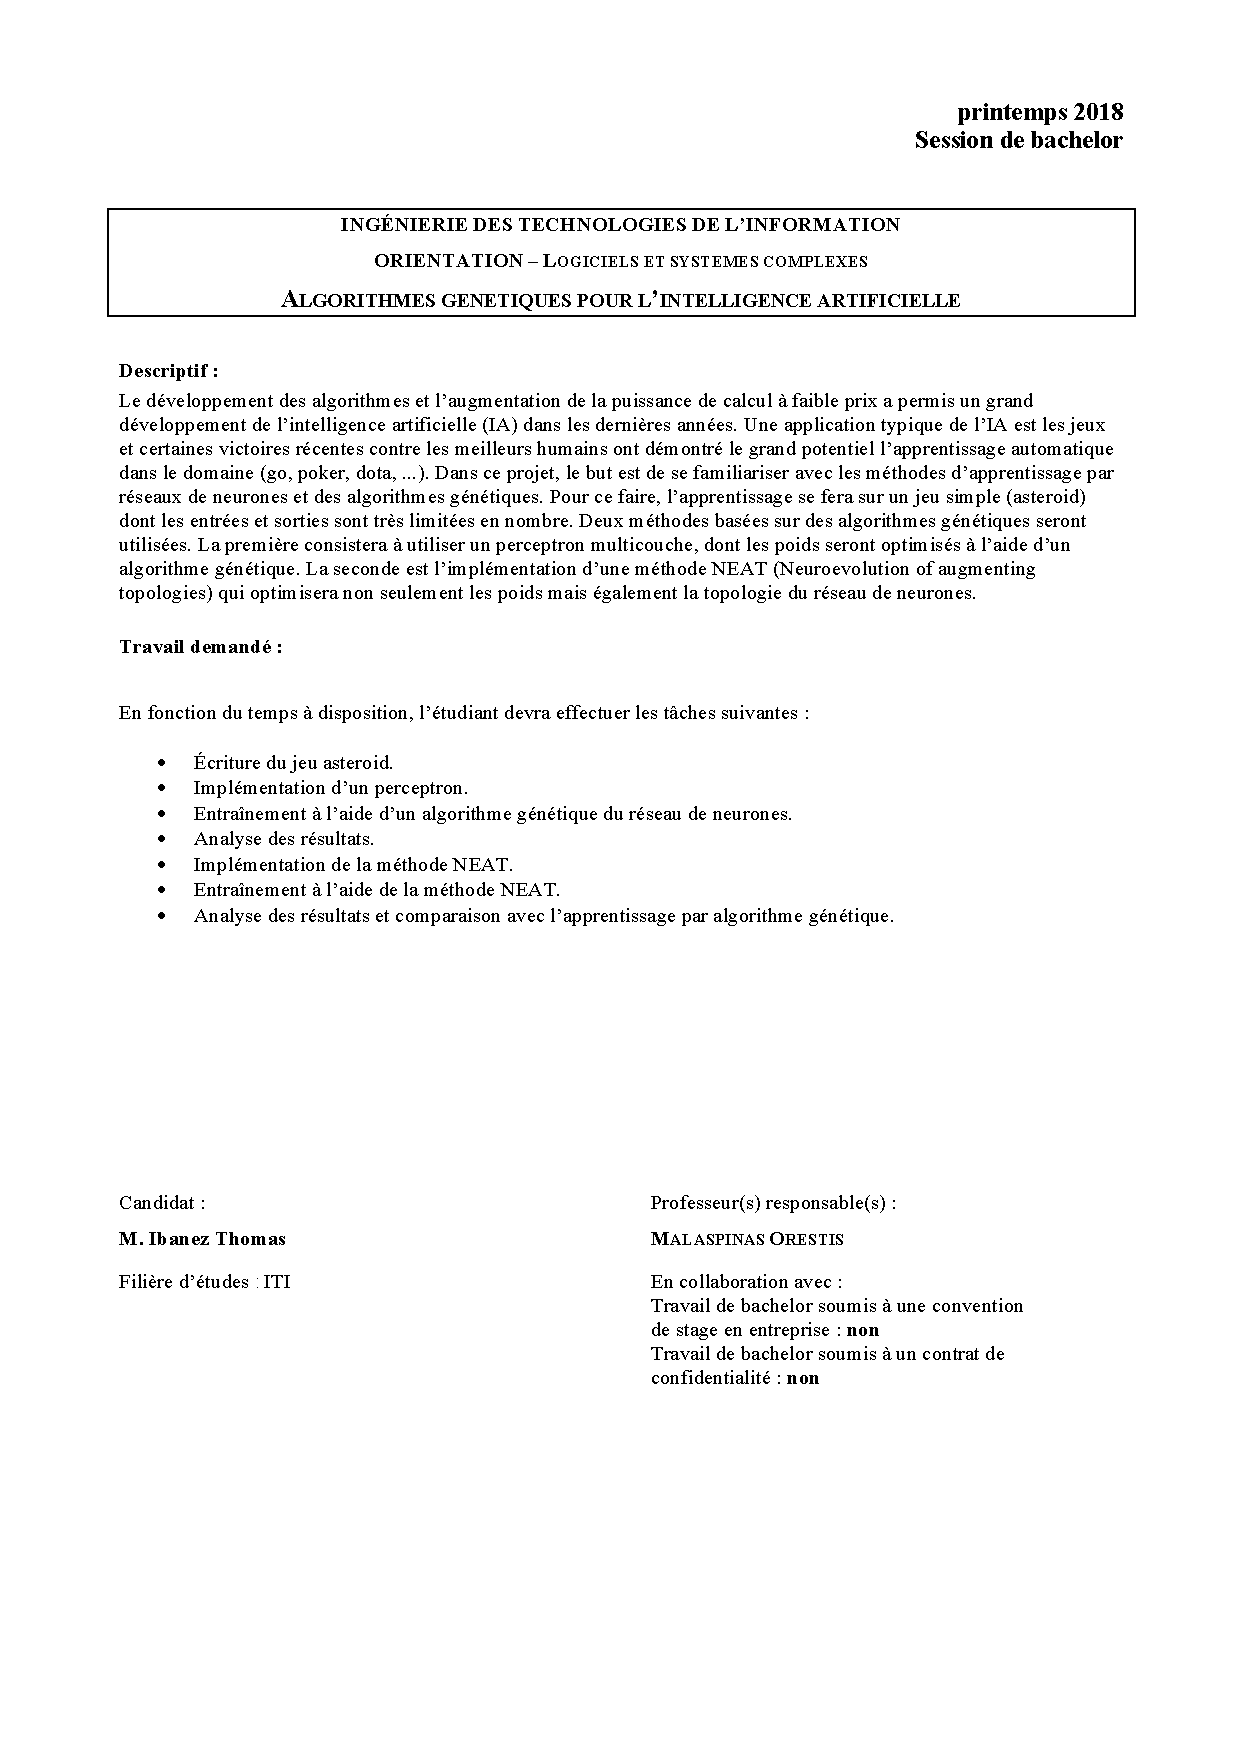
\includepdf[pages=1, offset=2cm 0]{enonce}

\tableofcontents

\newpage

\listoffigures

\newpage

\section*{Remerciements}
\section*{Acronymes}
IA
NEAT


\newpage
\section{Introduction}

Ces dernières années l'apprentissage automatique (Machine Learning) à pris une place très importante dans le monde de l'informatique et nous avons pu assister au prouesses accomplies par des intelligences artificielles tels que la victoire d'AlphaGo face à Lee Sedol au jeu de Go en 2016.\cite{wikialphagolee} Cet événement n'est pas sans rappeler la défaite de Kasparov contre Deep Blue en 1997 qui avait défrayé le chronique.\cite{kasparov}\\
Mais comment en sommes nous arrivés là, et quels sont les techniques qui se cachent derrière ces impressionnant résultats ?\\
Il y a plusieurs manière de faire du machine learning ; une des plus populaire, celle qui est utilisée pour ce travail, est le réseau de neurones artificiels. Cette technologie existe depuis bien longtemps, mais ce sont les récent progrès en terme de puissance de calcul qui ont amorcé sa montée comme technologie phare du domaine.\cite{nnpower}\\

La méthode classique pour entrainer des réseaux de neurones est la rétropropagation du gradient (backpropagation). Cette technique consiste à comparer la sorties du réseau à la sortie attendu pour une entrée donnée afin de corriger les poids du réseau.\cite{backprop} L'avantage de cette technique est qu'elle va converger très rapidement vers le résultat attendu (à condition que les hyperparamètres du réseau soit adaptés au problème). Le désavantage est qu'il faut avoir à sa disposition un grand nombres d'entrées dont on connait la nature afin de pouvoir les comparer aux résultats du réseau. Par exemple il existe une base de données de chiffres écrit à la main avec leur valeur réelle sur \url{http://yann.lecun.com/exdb/mnist/} (70'000 entrées).\\

Cependant générer une telle base de données est un travail énorme, ainsi ces dernières années nous avons assisté à l'émergence de nouvelles technique ne nécessitant pas d'exemples.\\

Une de ces techniques, qui a été utilisée pour l'apprentissage d'AlphaGo\cite{alphago}, est le l'apprentissage par renforcement (Reinforcement learning). Cette méthode consiste à juger les décisions prises par un agent autonome en lui donnant une recompense positive ou négative afin que l'agent, au fur et à mesure des expériences trouve une stratégie optimale.\cite{wikirl} Cette façon de faire peut être comparé au comportement d'un enfant qui apprends à faire du vélo. Quand il tombe il va avoir mal, c'est une récompense négative. Il va donc corriger son comportement de façon à ne plus tomber. A l'inverse, quand il arrive a aller loin il va être fier et donc favoriser ce comportement, c'est une récompense positive.\\

Cependant il existe une méthode encore plus généraliste pour l'apprentissage: La neuroévolution. Cette méthode se base sur les algorithmes évolutionniste dont le fonctionnement est inspiré de la sélection naturelle qui a guidé l'évolution de la vie sur terre. En effet à partir d'un ensemble d'organismes que nous allons évaluer à leur capacité effectuer une tâche donnée, ce que nous appelons le \textit{fitness} de l'organisme. Nous allons sélectionner les meilleurs d'entre eux afin de les faire se "reproduire" pour créer la génération suivante qui sera à son tour évaluée et on recommence ce processus autant de fois que nécessaire.\cite{wikineuroevolution}\\

Le but de ce travail de bachelor est d'étudier et de comparer le comportement deux algorithmes de neuroévolution en analysant la faculté de chacun à apprendre à jouer à des jeux vidéo. Cette technique à été choisie car elle permet un développement plus libre de l'IA en ne jugeant que le résultat et non pas les actions qui y mène.
\newpage

\section{Agent Intelligent}

Un agent intelligent est une entité autonome qui observe son environnement grâce à des capteurs et qui peut agir sur l'état de son environnement grâce à des effecteurs. Cette entité doit avoir un objectif, elle peut également apprendre où utiliser ses connaissances pour atteindre son but.\cite{wikiia}\\

\begin{figure}[H]
\begin{center}
	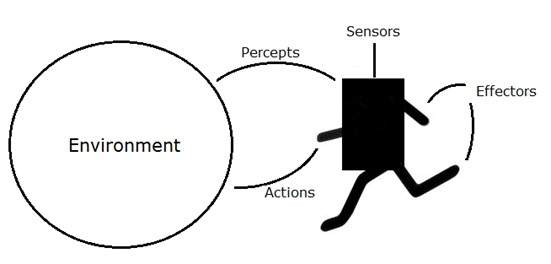
\includegraphics[scale=0.5]{agent_environment.jpg}
	\caption{Illustration d'un agent}
\end{center}
\end{figure}

\subsection{Mesure de la performance}

La mesure de la performance est un critère qui va définir l'efficacité d'un agent, ce critère dépend évidement de la tâche demandée à l'agent. Cette mesure est analogue à la mesure de la valeur sélective (fitness) d'un organisme en biologie. Ainsi si le tâche demandée à l'agent est de séparer les M\&M's bleu des M\&M's rouges, sa performance peut être mesurée par son taux d'erreur et sa rapidité.

\subsection{Rationalité}

La rationalité est le fait d'être raisonnable, sensible et d'avoir un bon sens du jugement.\\
Un agent rationnel va toujours effectuer la "bonne" action, celle qui va apporter le plus de succès à l'agent par rapport à la séquence perçue.\cite{tutoptai}

\subsection{Environnement}

L'environnement peut être de différentes natures en fonction du problème pour lequel l'agent est déployé.

\subsubsection{Discret / Continu}

Si les états possibles de l'environnement sont dénombrables et clairement définis, l'environnement est dit "discret". Par exemple le jeu de Go est un environnement discret car on peut lister tout les états possibles du plateau. En revanche un simulateur de conduite est continu, on ne peut pas lister toutes les positions possible de la voiture.\cite{tutoptai}

\subsubsection{Observable / Partiellement Observable}

L'environnement est observable si l'agent peut à tout moment en observer la totalité, sinon l'environnement est partiellement observable. Par exemple le jeu DotA 2 n'est que partiellement observable car du brouillard cache une partie de l'environnement.\cite{tutoptai}

\subsubsection{Statique / Dynamique}

Si l'environnement ne change pas tant qu'un agent n'agit pas, il est dit statique. Sinon il est dynamique. Un exemple d'environnement statique est le jeu du monopoly, tant qu'un joueur n'agit pas l'état du jeu ne change pas. Au contraire dans les flippers, la balles va continuer à bouger même si le joueur ne fait rien.\cite{tutoptai}

\subsubsection{Simple agent / Multi-agents}

Lorsque l'environnement n'est influencé que par un seul agent il est dit simple agent, c'est la cas du jeu space invaders qui se joue seul. Si l'environnement est influencé par plusieurs agents il est dit multi-agents, la planète terre est donc un environnement multi-agents.\cite{tutoptai}

\subsubsection{Déterministe / Non-déterministe}

L'environnement est dit déterministe si on peut prévoir, à partir d'une observation de l'état actuel de l'environnement, l'état suivant de l'environnement. Autrement dit si l'aléatoire n'intervient pas dans l'évolution de l'environnement alors il est déterministe.\cite{tutoptai}

\subsubsection{Épisodique / Non-épisodique}

Un environnement épisodique est divisé en épisodes, un épisode est une série d'observation qui mène à une et une seule action, une fois l'action effectuée l'épisode est terminé. Ainsi les actions et décisions passée de l'agent (les épisodes passés) n'ont aucune influence sur l'état actuel de l'environnement.\\
Un exemple d'environnement épisodique est un agent qui regarde des images pour les classer, une fois le choix fait celui-ci n'aura pas d'influence sur les images suivantes. Au contraire dans un jeu comme le jeu d'échecs, chaque coup dépends du coup précédent, c'est donc un environnement non-épisodique.\cite{tutoptai}

\newpage
\section{Réseau de Neurones Artificiels}

Un réseau de neurones est un modèle, inspiré du fonctionnement du cerveau humain, qui va consister en un ensemble de neurones artificiels (aussi appelés perceptrons), disposés en couches qui vont communiquer en propageant une information.\cite{wikiann} En effet les neurones de notre cerveau vont collecter les signaux en provenance de leurs dendrites, puis si les signaux sont assez fort envoyer une impulsion le long de leur axone vers les neurones suivant qui vont faire de même. A noter que les connexions entre deux neurones peuvent être plus ou moins fortes (le signal va donc se propager avec une intensité variable).\cite{neuronswork}

\begin{figure}[H]
\begin{center}
	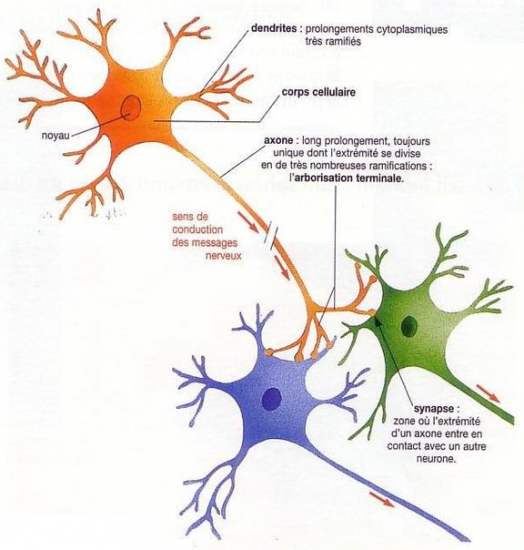
\includegraphics[scale=0.5]{neurones.png}
	\caption{Représentation des neurones dans le cerveau humain \cite{neurons}}
\end{center}
\end{figure}

Les perceptrons quant à eux vont imiter (de manière simplifiée) ce comportement, chaque perceptron va prendre le signal envoyée par chacun de ses voisins de la couche précédente, puis multiplier cette valeur par le poids le connexion et finalement faire le somme de toutes les valeurs pondérées et passer cette somme dans une fonction (dites fonction d'activation) qui va placer cette somme dans un interval (entre 0 et 1 par exemple) et renvoyer le résultat de cette fonction à tous ses voisins de la couche suivante qui vont faire de même.\cite{wikiperceptron}

D'un point de vue mathématique le comportement d'un perceptron peut être écrit comme:
\begin{equation}
o = f(\sum_{i=0}^{n} S_i * W_i)
\label{eq:percep}
\end{equation}
Où\\
$o$ est le signal qui va sortir du perceptron\\
$f$ est la fonction d'activation\\
$n$ est le nombre de voisins de la couche précédente\\
$S$ est le vecteur des signaux des voisins la couche précédente\\
$W$ est le vecteur des poids entre le perceptrons et ses voisins de la couche précédente

\begin{figure}[H]
\begin{center}
	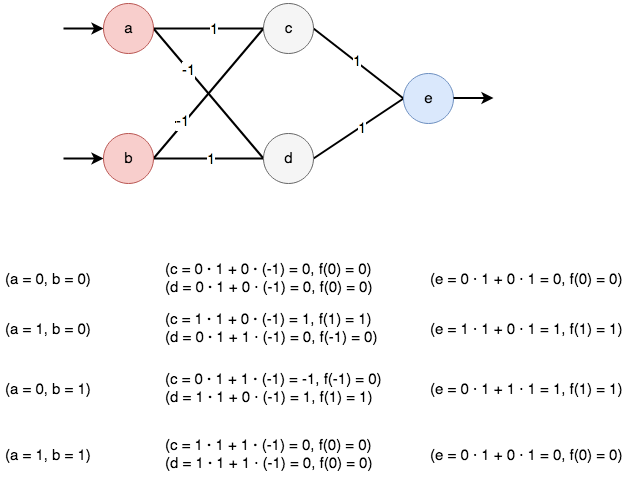
\includegraphics[scale=0.7]{xor.png} 
	\caption{Porte logique "ou exclusif" (XOR) simulée par un réseau de neurones}
\end{center}
\end{figure}

Les neurones de la première couche vont recevoir leurs valeur depuis l'extérieur. Ces entrées (aussi appelées \textit{features}) dépendent du problème pour lequel le réseau est employé. Ainsi si nous cherchons à prédire le note d'un examen en fonction du temps de révision et de nombre d'heures de sommeil, les entrées du réseau seront le temps de révision et le nombres d'heures de sommeil.\\
 Chaque neurones de la couche suivante calculera sa valeur par propagation du signal de la couche précédente afin d'arriver jusqu'à la dernière couche de neurones qui déterminera la prédiction du réseau de neurones. Cette prédiction est également appelée \textit{label}. Dans le cas de notre exemple, le label du réseau sera la note prévue.\\
 Avant de pouvoir utiliser notre réseau pour faire des prédictions, il faut l'entrainer, c'est à dire ajuster les paramètres (poids, topologie) afin que les labels soient le plus correct possible pour des features données.\\
 
\begin{figure}[H]
\begin{center}
	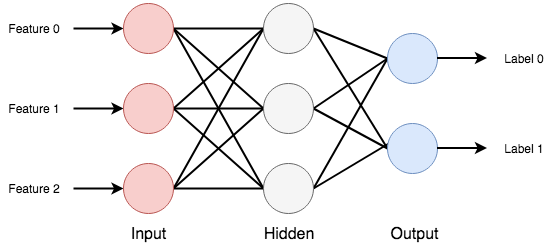
\includegraphics[scale=0.7]{ff.png}
	\caption{Réseau de neurones}
\end{center}
\end{figure}
 
 Il est cependant important de ne pas mystifier le fonctionnement des réseaux de neurones. Ce sont certes des "boites noires", c'est à dire qu'il n'est pas possible d'analyser un réseau et d'expliquer pourquoi une connexion donnée a un tel poids. En revanche, il ne faut pas perdre de vue que leur comportement est exprimable par une fonction mathématique. En effet tout comme le comportement d'un perceptron est décrit dans l'équation \ref{eq:percep} le comportement de n'importe quel réseau de neurones peut-être décrit par une equation dépendant du réseau.

\subsection{Apprentissage supervisé}

L'apprentissage supervisé est une manière d'entrainer un réseau de neurones avec un ensemble de couples (features, labels). Le but est de commencer avec un réseau initialisé aléatoirement, puis de lui donner en entrée des features dont le labels sont connu et de comparer les labels donnés par le réseaux aux labels attendus.\\
En fonction du taux d'erreur, il sera possible de corriger les poids des connexions du réseau pour minimiser ce taux.\cite{wikisupervised}\\

Les avantages principaux de cette technique d'apprentissage sont la rapidité d'entrainement et la justesse atteignable étant donné que le fonctionnement ne dépend pas d'heuristiques.\\

Les désavantages sont le temps de génération de la base d'exemples et le fait qu'il faille connaitre le label attendu pour chaque feature (nous savons à coup sur qu'une image de chien doit être classifiée comme "chien" mais nous ne savons pas le coup idéal à jouer selon l'état d'un plateau de jeu).

\subsection{Apprentissage non supervisé}

L'apprentissage non supervisé est une méthode d'apprentissage où l'entrainement se fait avec un semble de features dont le label n'est pas connu. Une utilisation de cette technique est le partitionnement de données où le réseau va apprendre à regrouper des features similaires dans la même catégorie.\cite{wikiunsupervised}\\

Cette méthode peut être comparée à la manière dont un enfant apprends à reconnaître son environnement, si il voit 50 voitures il va pouvoir les associer comme étant des object similaires, sans pour autant qu'on ai eu besoin de lui expliqué ce qu'est un voiture.

\subsection{Apprentissage par renforcement}

L'apprentissage par renforcement intervient lorsque qu'on veut optimiser les décisions prise par un agent intelligent en fonction de son environnement, il est possible que l'agent soit controlé par un réseau de neurones. Dans ce cas les décisions seront les labels et les informations sur son environnement seront les features. Le concept de l'apprentissage par renforcement est de récompenser ou de pénaliser les choix fait par l'agent afin qu'au fur et à mesure des expériences il optimise son comportement.\cite{wikirl}

\subsection{Neuroevolution}

La neuroévolution en est une technique d'entrainement dont le but est d'utiliser les principes des algorithmes évolutionnistes afin d'optimiser un réseau de neurones pour effectuer la tâche désirée. A la différence de l'apprentissage par renforcement, ce ne sont pas les actions individuelles qui vont être jugée mais l'efficacité totale du réseau. Nous ne cherchons donc pas à développer un comportement particulier mais juste à entre plus optimal, peut importe la manière.\cite{wikineuroevolution}\\

\subsection{Fonctions d'activation}

Les fonction d'activations sont des fonctions qui ont pour tâche de limiter la valeur des neurones dans un interval donné. Afin de pouvoir appliquer la rétropropagation du gradient il faut également que la fonction soit dérivable.
Voici quelques exemples de fonctions utilisées couramment:\\

La sigmoid $\sigma : \mathbb{R} \rightarrow ]0, 1[$
\begin{equation}
	\sigma : x \mapsto \frac{1}{1 + e^{-\beta x}}
\end{equation}

\begin{figure}[H]
\begin{center}
	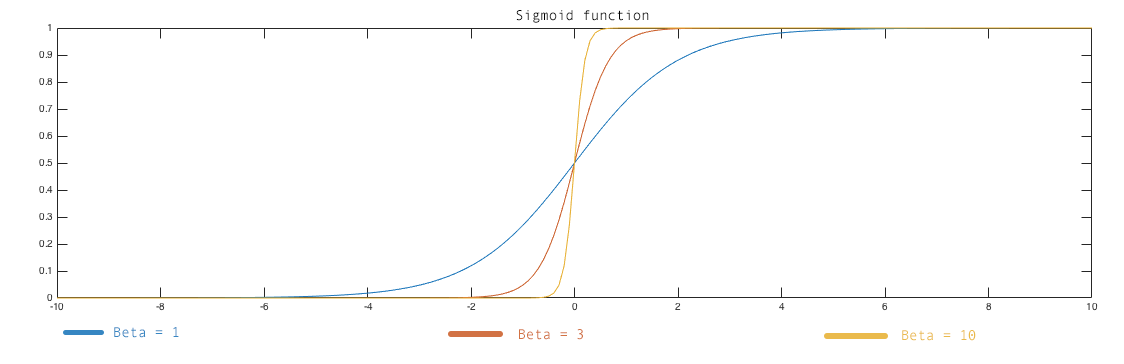
\includegraphics[scale=0.4]{sigmoid.png} 
	\caption{Fonction Sigmoid avec des $\beta$ variables}
\end{center}
\end{figure}

La tangente hyperbolique $tanh : \mathbb{R} \rightarrow ]-1, 1[$
\begin{equation}
	tanh : x \mapsto \frac{e^x - e^{-x}}{e^x + e^{-x}}
\end{equation}

\begin{figure}[H]
\begin{center}
	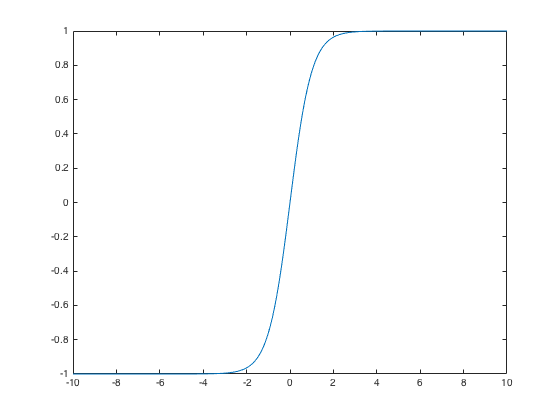
\includegraphics[scale=0.4]{tanh.png} 
	\caption{Fonction tangente hyperbolique}
\end{center}
\end{figure}

La fonction step $step : \mathbb{R} \rightarrow [0, 1]$
\begin{equation}
	step : x \mapsto
		\begin{cases}
			0, & \text{if}\ x \leq 0\\
			1, & \text{otherwise}
		\end{cases}
\end{equation}

\begin{figure}[H]
\begin{center}
	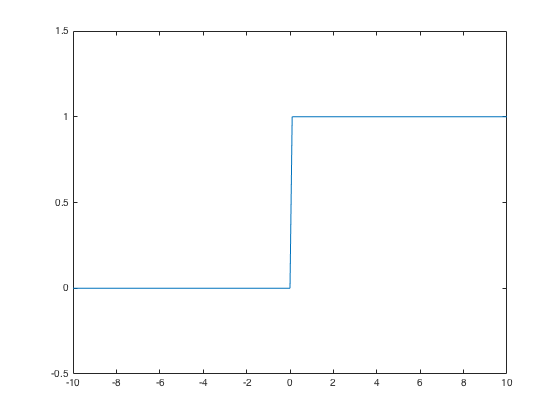
\includegraphics[scale=0.4]{step.png} 
	\caption{Fonction step}
\end{center}
\end{figure}

\newpage
\section{Algorithmes évolutionnistes}

Un algorithme évolutionniste est un algorithme d'optimisation métaheuristique qui cherche, par un processus inspiré de la sélection naturelle, une solution optimale à un problème. Ces algorithmes utilisent des iterations stochastiques pour arriver à maximiser une fonction évaluant leurs performances, dite fonction de fitness.\cite{wikiea}\\

\subsection{Génome \& Phénome}

Le génome est l'ensemble du matériel génétique d'un individu, celui-ci contient toutes les informations nécessaire à la création de l'individu.\cite{wikigenome} Chez les humain le génome est organisé en 23 paires de chromosomes. A partir de ces chromosomes, qui sont uniques à chaque organismes, on peut créer le phénome.\\
Le phénome est l'ensemble de tout les traits observables chez un individu (p.ex La couleur des yeux, de la peau, des cheveux etc...).\cite{wikiphenome}\\

Dans le cadre de la neuroévolution le génome est un encodage permettant la création du phénome qui est le réseau de neurones.

\subsection{Population initiale}

La base d'un algorithme évolutionniste est la population initiale, celle-ci doit être générée aléatoirement afin de représenter un vaste spectre de possibilités. 
Nous ne retrouverons dans cette population aléatoire aucuns individu capable d'accomplir parfaitement la tâche demandée, mais certains aurons des comportements qui les aiderons a d'obtenir un fitness plus élevé que leurs voisins, ceux-ci vont donc passer leurs caractéristiques à la génération suivante.

\subsection{Sélection}

La sélection est un concept essentiel dans l'utilisation d'algorithmes évolutionnistes. L'objectif est de choisir, en prenant en compte le fitness afin que les individus performant soit plus souvent sélectionnés pour être parents. Ainsi, les caractéristiques qui les rendent plus performant seront plus largement passés vers la génération suivante alors que les caractéristiques des individus plus faibles disparaîtront rapidement.\cite{wikifps}

\begin{figure}[H]
\begin{center}
	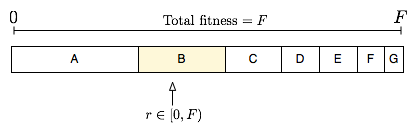
\includegraphics[scale=0.6]{fps.png} 
	\caption{Exemple de sélection proportionnelle au fitness\cite{wikifps}}
\end{center}
\end{figure}

\subsection{Crossover}

Un crossover (où enjambement en français) est une opération génétique qui croise les gènes de deux parents afin de créer le gène de l'enfant, ce dernier va donc hériter de certaines caractéristiques de l'un où l'autre parent. Un exemple visible de cette opération chez les humains est que l'on reconnait des traits (couleur de peau, yeux, cheveux) des parents chez les enfants.\cite{wikicrossover}\\

\subsection{Mutation}

Les mutations sont des événements aléatoires qui vont altérer le génome de façon à créer une innovation, qui va par exemple se traduire par un comportement différent du génome. Dans certains cas les mutations seront bénéfiques (p.ex La capacité à respirer hors de l'eau), dans d'autre la mutation causera un comportement désavantageux (p.ex Malformation des membres).\cite{wikimutation}\\

\subsection{Elitisme}

L'Elitisme est un concept qui va permettre la survie des meilleurs individus d'une génération vers la génération suivante sans que leur code génétique soit modifié.\cite{elitism}\\
La raison pour laquelle ce concept est mis en place est que les solutions optimales trouvées ne doivent pas être perdues à cause de mutations désavantageuses.


\newpage
\section{Evolution du perceptron multicouche - Algorithme Naïf}

Cette section détaille le fonctionnement de l'algorithme évolutionniste mis en place pour faire évoluer les perceptrons multicouche à topologie fixe. Celui-ci va donc uniquement faire varier les poids des connexion dans le réseau pour optimiser son comportement. L'algorithme à été créé en s'inspirant des concepts d'algorithmes évolutionnistes décrit précédemment.

\subsection{Génome \& Phénome}

Pour cet algorithme le génome est simplement la liste des poids constituant le réseau de neurones. Ainsi, étant donne que la topologie du réseau est fixe, on peut le reproduire à l'identique en assignant les bons poids.\\

Le phénome dans le cas de cet algorithme sera une réseau de neurones à topologie fixe et entièrement connecté (Chaque neurones d'une couche donnée est connecté a chaque neurones de la couche suivante).

\begin{figure}[H]
\begin{center}
	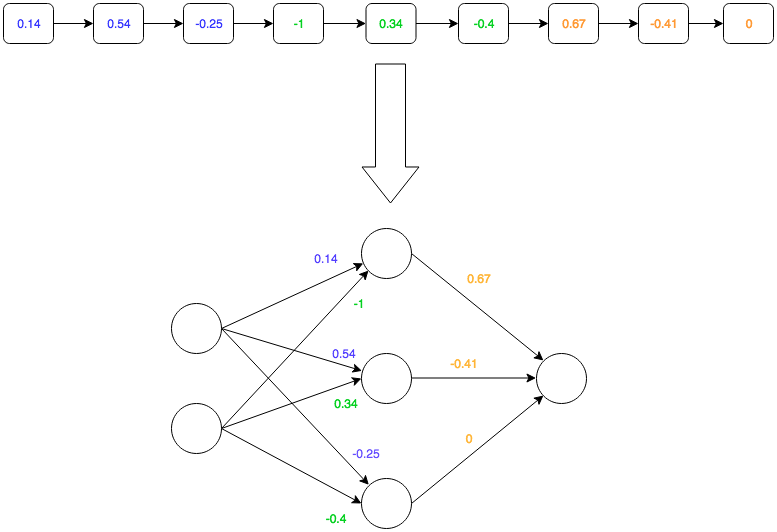
\includegraphics[scale=0.5]{genomephenome.png}
	\caption{Passage du génome au phénome}
\end{center}
\end{figure}

\subsection{Population initiale}

La population initiale est un ensemble de perceptrons multicouche dont la topologie est la même, les poids entre les couches sont assignés aléatoirement à une valeur entre -1 et +1 afin de représenter un spectre de possibilités aussi large que possible.
\begin{figure}[H]
\begin{center}
	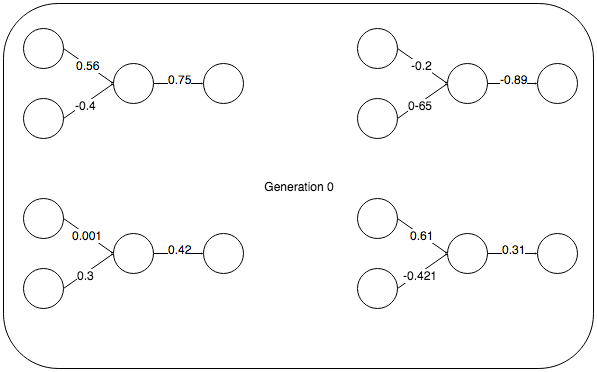
\includegraphics[scale=0.6]{gen0mlp.png} 
	\caption{Exemple de population initiale}
\end{center}
\end{figure}

\subsection{Sélection}

La sélection est utilisée pour choisir un individu de la génération précédente qui va soit passer ses gènes directement (être cloné), soit faire un crossover avec les gènes d'un autre individu lui aussi sélectionné. La probabilité de l'une ou l'autre de ces actions est de 50\%.\\
Le génome résultant de cette sélection subira ensuite une potentielle mutation. Ce processus est répété autant de fois que nécessaire pour créer une nouvelle génération contenant autant d'organismes que la précédente.

\subsection{Crossover}

Le crossover fonctionne d'après un principe très simple:\\
\begin{itemize}
\item Choisir un point de croisement
\item Assigner chez l'enfant tout les gènes qui précèdent ce point depuis le premier parent
\item Assigner chez l'enfant tout les gènes qui suivent ce point depuis le second parent
\end{itemize}

\begin{figure}[H]
\begin{center}
	\includegraphics[scale=0.6]{"crossover.png"} 
	\caption{Fonctionnement d'un crossover}
\end{center}
\end{figure}

Ainsi, les traits permettant une meilleure survie vont rapidement se répandre dans la population car les individus ayant obtenu un meilleur fitness serons plus souvent sélectionnés pour faire une crossover avec un autre individu.

\subsection{Mutation}

Dans le cas de cet algorithme, étant donné que la topologie est fixe, la mutation sera simplement une variation aléatoire d'un poids dans le réseau de neurones. Ainsi chaque enfant de chaque génération aura 10\% de chance que l'un de ses gènes subisse une mutation.\\
Le poids subira donc une variation d'une valeur aléatoire choisie entre +0.5 et -0.5 cependant le poids sera ensuite fixée dans l'interval $[-1, 1]$.

\begin{figure}[H]
\begin{center}
	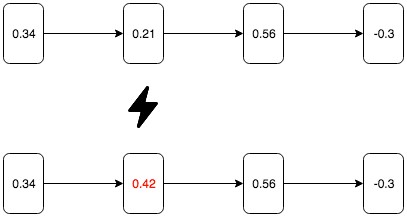
\includegraphics[scale=0.6]{mutation.png}
	\caption{Exemple de mutation dans un génome}
\end{center}
\end{figure}

\subsection{Elitisme}

Pour cet algorithme, seul le champion de la génération (organisme ayant obtenu le meilleur fitness) est préservé sans altération de son code génétique pour la génération suivante.

\begin{figure}[H]
\begin{center}
	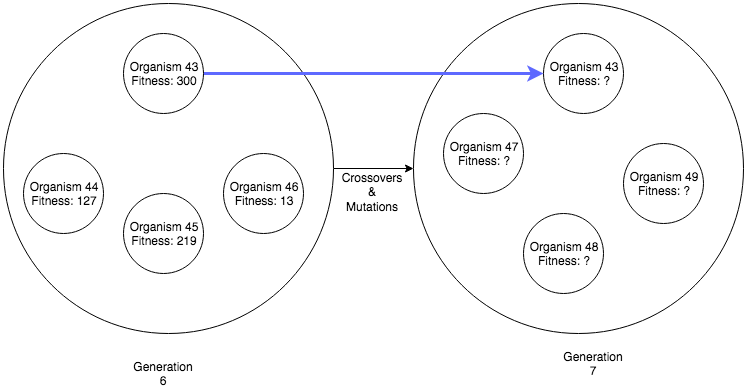
\includegraphics[scale=0.5]{elitism.png}
	\caption{Elitisme d'une génération vers la suivante}
\end{center}
\end{figure}

\subsection{Déroulement de l'algorithme}

L'organigramme ci-dessous décrit le comportement global de l'algorithme. La fonction random(0, 1) va tirer un nombre aléatoire entre compris dans l'interval $[0, 1[$.
\afterpage{%
\begin{figure}[H]
\centering
\vspace*{-3cm}
\thispagestyle{empty}
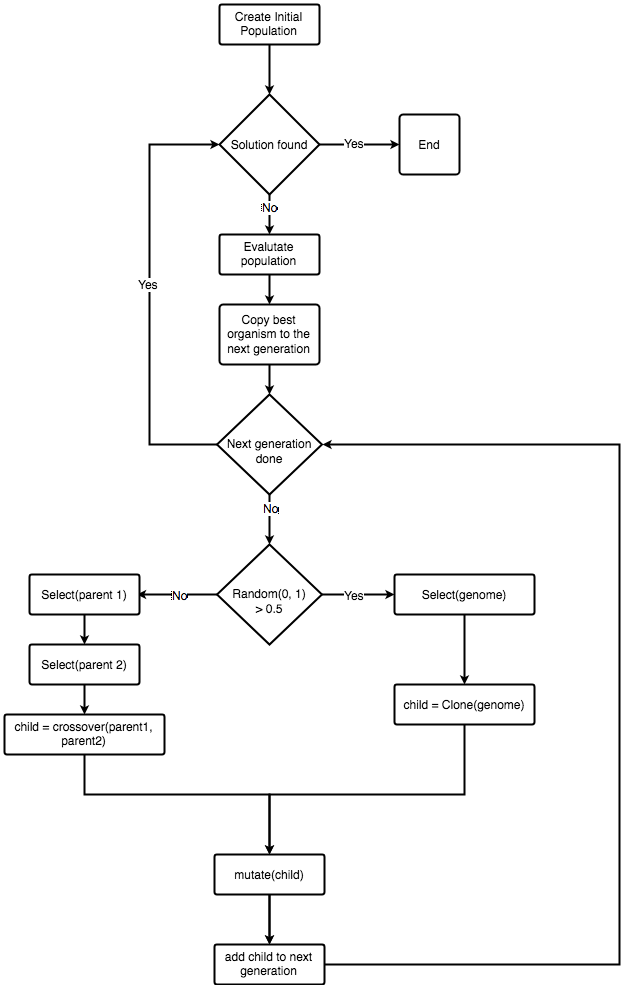
\includegraphics[scale=0.6]{mlporga.png}
\caption{Organigramme de l'algorithme naïf}
\end{figure}
\clearpage
}
\newpage

\section{NEAT}

L'autre algorithme de neuroévolution mis en place est le NEAT, créé par Ken Stanley à Université du Texas à Austin. Cet algorithme détaille comment obtenir des réseaux de neurones dont la topologie change au fil des évolutions.\\
Il apporte trois techniques essentielles à son fonctionnement: suivre l'évolution des gènes avec un historique pour permettre les crossover parmi les différentes topologies, séparer les organismes en espèces afin de préserver l'innovation et faire évoluer les topologies de manière incrémentale en partant de structures simples afin d'obtenir des résultats minimaux.\cite{wikineat}

\subsection{Génome \& Phénome}

Dans le cas de NEAT, le génome est plus complexe, en effet il doit représenter tout les neurones et toutes les connexions. Etant donné que le réseau n'est pas forcément entièrement connecté, et que les connexions peuvent "sauter" des couches, le génome est constitué de deux listes, une qui représente tout les neurones du réseau et une qui représente toutes les connexions du réseau. 

\begin{figure}[H]
\begin{center}
	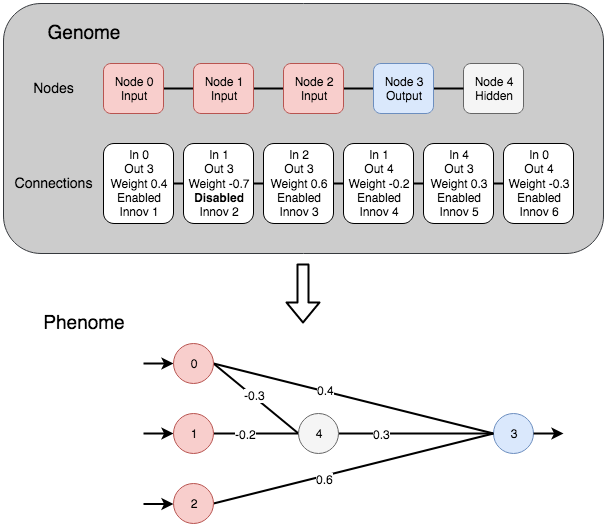
\includegraphics[scale=0.55]{genomephenomeneat.png}
	\caption{Passage du génome au phénome dans NEAT}
\end{center}
\end{figure}

\subsection{Population initiale}

La population initiale doit être aussi simple que possible, cependant il n'y a pas de règles dictant la manière dont elle doit être faite. Pour cet algorithme, la population initiale est donc un ensemble de perceptron multicouche avec seulement une couche d'entrée et une couche de sortie dans lequel chaque entrée est reliée à chaque sorties.

\begin{figure}[H]
\begin{center}
	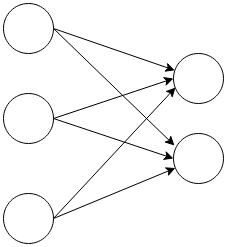
\includegraphics[scale=0.6]{initneat.png}
	\caption{Exemple de population initiale dans NEAT}
\end{center}
\end{figure}

Ce choix à été fait pour conserver un équilibre entre une population simple (pas de couche intermédiaire) mais qui soit rapidement capable de s'ajuster car les connexions sont déjà disponibles, on ne pert donc pas de générations uniquement pour créer les connexions.

\subsection{Historique des innovations}

Une innovation est l'apparition dans le génome d'une nouvelle connexion. Un points central de l'algorithme est de suivre l'émergence de ces innovations afin d'étiqueter les innovations semblables par un même numéro. Ainsi si nous avons deux réseau ayant la même topologie qui, l'un après l'autres font apparaitre une nouvelle connexion entre les mêmes noeuds, leurs deux connexions auront le même numéro d'innovation.\\
	
Afin de faire ce lien il faut d'abort faire une recherche pour savoir si cette connexion à déjà été ajoutée dans un autre réseau. Si oui, la connexion ajoutée prend le numéro d'innovation déjà existant. Sinon un nouveau numéro d'innovation est généré et on ajoute à l'historique des innovation sous le format suivant (numéro d'innovation, neurone d'entrée, neurone de sortie, innovations déjà présentes dans le génome).\\

\subsection{Spéciation}

Une particularité de NEAT est la séparation des organismes en espèces, l'objectif de cette séparation est de protéger les nouvelles topologies pour qu'elles ai le temps de se développer, et pénaliser les espèce ne s'améliorant pas avec le temps.\\ 

Pour effectuer cette spéciation, il faut comparer les similarités entre les génomes, plus particulièrement il faut aligner les gènes homologues (ayant le même numéro d'innovation) et compter les gènes dit \textit{disjoints} où \textit{excess}.\\
Un gène est dit disjoint si il n'apparait que dans un des deux génomes comparés mais que son numéro d'innovation est plus petit que le plus grand numéro d'innovation de l'autre génome. Un gène est dit excess si il n'apparait que dans un des deux génomes comparés mais que son numéro d'innovation est plus grand que le plus grand numéro d'innovation de l'autre génome. Les gènes qui ne sont ni disjoints ni excess sont dit \textit{matching}.

\begin{figure}[H]
\begin{center}
	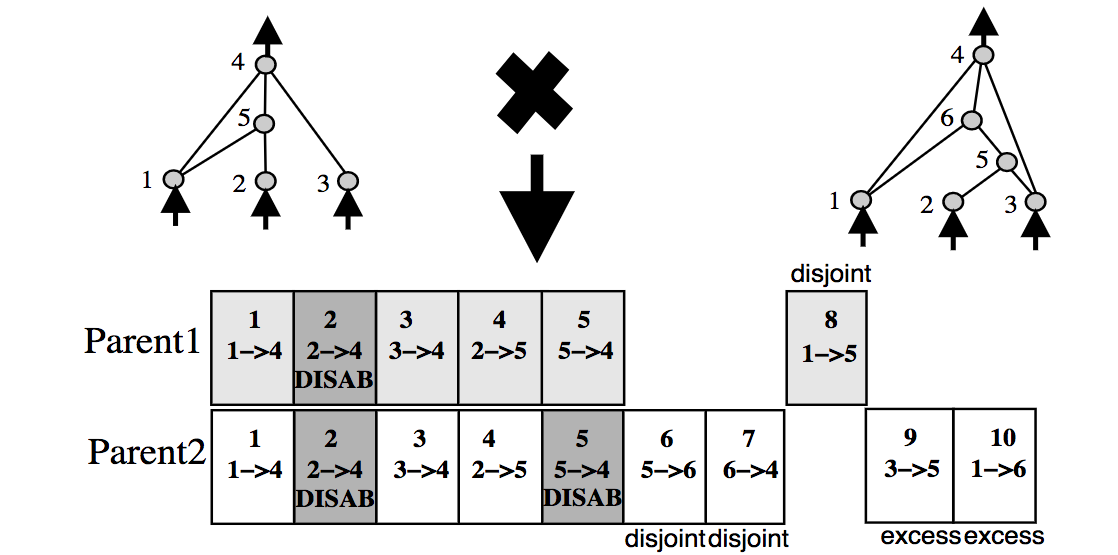
\includegraphics[scale=0.4]{disjointexcess.png}
	\caption{Comparaison de deux génomes dans NEAT.\cite{neatpaper}}
\end{center}
\end{figure}

La dernière étape avant de pouvoir calculer la distance entre deux génomes est de calculer la moyenne des écarts entre les poids de chaque connexion.
La formule calculant la disparité entre deux génomes est la suivante:

\begin{equation}
	\delta = \frac{c_1 * E}{N} + \frac{c_2 * D}{N} + c_3 * \overline{W}
\label{eq:delta}
\end{equation}

Où\\
$c_1$ est le coefficient d'excess\\
$E$ est le nombre de gènes excess\\
$c_2$ est le coefficient de disjoints\\
$D$ est le nombre de gènes excess\\
$N$ est le nombre total de gènes, peut être assigné à 1 si le réseau est petit (moins de 20 connexions)\\
$c_3$ est le coefficient de l'écart des poids\\
$\overline{W}$ est la moyenne des écarts des poids\\

Les coefficients peuvent être modifiés pour changer la sensibilité de la classification aux différents paramètres. Une fois la valeur de $\delta$ calculée, elle est comparée avec un seuil $\delta_t$, si la valeur est plus grande, les génomes ne font pas partie de la même espèce, sinon ils font partie de la même espèce.\\

Afin de préserver l'innovation et d'éviter qu'une espèce domine rapidement la totalité de la population, un mécanisme de \textit{fitness sharing} est mis en place. Pour ce faire le fitness de chaque organisme d'une espèce est divisé par le nombre d'organisme dans cette espèce. Ainsi, les petites espèce qui émergent d'une innovation topologique seront protégées de l'extinction pendant quelques génération afin de laisser le temps aux organismes de s'ajuster.\\

Plus formellement le fitness ajusté de l'organisme $i$ $f^\prime_i$ est défini comme:

\begin{equation}
	f^\prime_i = \frac{f_i}{\sum^n_{j=1} sh(\delta(i,j))}
\end{equation}
Où\\
$f_i$ est le fitness non ajusté de l'organisme i\\
$n$ est le nombre d'organismes\\
$sh$ est la fonction de sharing, celle si renvoie 0 quand son paramètre est inférieur à $\delta_t$ et 1 sinon\\
$\delta$ est la fonction comparant les génomes vue dans l'équation \ref{eq:delta}\\

\subsection{Sélection}

Dans NEAT, la sélection intervient au moment de la création d'une nouvelle génération, cette sélection va d'abort être effectuée sur les espèce, en effet les organismes faisant partie de la moitié la moins performante de chaque espèce vont être supprimés.\\
Ensuite les espèce dont le meilleur organisme ne s'est pas amélioré depuis 15 générations sont supprimées.\\
Pour finir chaque espèce $i$ se voit attribuée un nombre d'enfants $n_i$ calculé selon la formule suivante:
\begin{equation}
	n_i = \left\lfloor\frac{\overline{sf_i}}{pop * \sum^m_{j=1} \overline{sf_j}}\right\rfloor
\end{equation}
Où\\
$\overline{sf_i}$ est la moyenne des fitness des organismes de l'espèce i\\
$m$ est le nombre d'espèces\\
$pop$ est le nombre total d'organismes\\

Si le nombre d'enfant d'une espèce est inférieur à un, l'espèce disparait. Sinon l'espèce va produire n enfants dans la génération suivante en utilisant le principe de la sélection proportionnelle au fitness. En effet lors de la création d'un enfant il y a 25\% de chance que l'enfant soit une copie d'un parent sélectionné et 75\% de chance que l'enfant soit le fruit d'un crossover entre deux parents sélectionnés (il subira dans les deux cas une potentielle mutation).

\subsection{Crossover}

Le crossover dans NEAT est fait pour palier au problème des conventions concurrentes (competing conventions). En effet il possible que deux réseaux produisent le même résultat mais de manière différente, le risque est que lorsque nous croisons les deux réseau nous perdions une partie de l'information qui les rends efficace.

\begin{figure}[H]
\begin{center}
	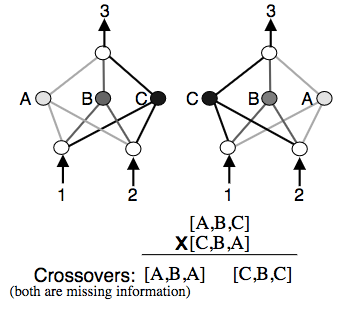
\includegraphics[scale=0.7]{competingconventions.png}
	\caption{Problème des conventions concurrentes, les deux réseaux atteignent le même résultat mais leurs possibles enfants en n'aurons que 2/3 de l'information \cite{neatpaper}}
\end{center}
\end{figure}

Pour palier à ce problème, il faut que seul les éléments qui divergent entre deux génomes soit échanger et que les éléments similaires soit conservés.\\

Le crossover dans NEAT se fait en alignant tout les gènes homologues (ayant le même numéro d'innovation), pour chaque gène alignés il faut choisir aléatoirement de prendre celui du parent 1 ou du parent 2. Pour les gènes disjoint ou excess, seul ceux du parent ayant le fitness le plus élevé sont conservés.

\begin{figure}[H]
\begin{center}
	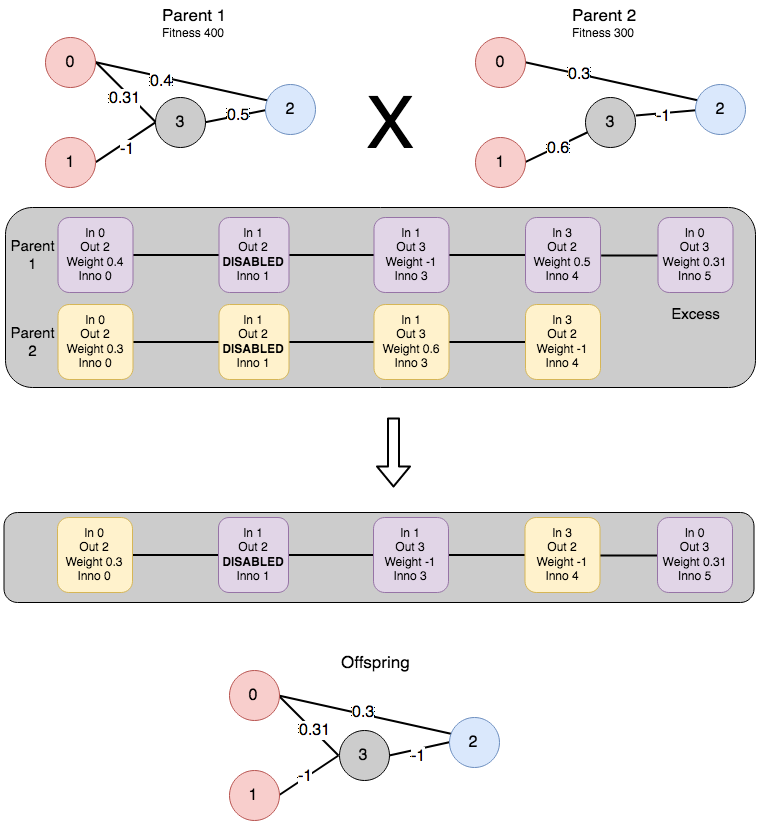
\includegraphics[scale=0.5]{crossoverneat.png}
	\caption{Crossover dans NEAT}
\end{center}
\end{figure}

\subsection{Mutation}

Les mutations dans NEAT peuvent être de trois types différents.

\subsubsection{Mutation de poids}

Une mutation de poids à 80\% de chance de se produire, si c'est le cas, tout les poids du réseau vont subir une mutation. Il y a 10\% de chance que le poids change totalement et 90\% de chance que le poids varie très légèrement.

\subsubsection{Mutation de connexion}

Une mutation de connexion consiste en l'ajout d'une connexion entre deux neurones n'étant pas déjà connectés et ne faisant pas partie de la même couche. Ce type de mutation à 5\% de chance de se produire.

\begin{figure}[H]
\begin{center}
	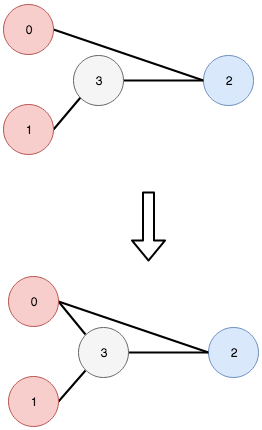
\includegraphics[scale=0.4]{addlink.png}
	\caption{Ajout d'une connexion}
\end{center}
\end{figure}

\subsubsection{Mutation de neurone}

Une mutation de neurone va ajouter un neurone dans le réseau, pour ce faire il faut choisir une connexion qui va être désactivée afin de la remplacer par deux connexions qui passent par le neurone ajouté. Cette mutation à 3\% de chance de se produire.

\begin{figure}[H]
\begin{center}
	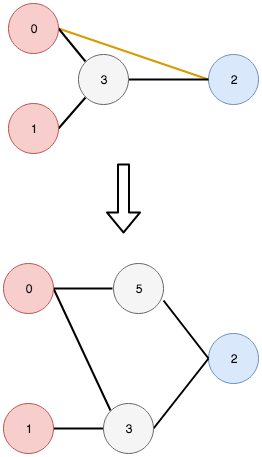
\includegraphics[scale=0.4]{addnode.png}
	\caption{Ajout d'un neurone}
\end{center}
\end{figure}

\subsection{Elitisme}

L'élitisme intervient dans l'algorithme car chaque espèce ayant au moins un enfant à créer va d'abort copier son champion de la génération passée sans lui faire subir de mutation vers la génération suivante.

\subsection{Déroulement de l'algorithme}

L'organigramme de l'algorithme NEAT se présente comme suit, il n'est pas possible de représenter en détaille toutes les opérations faites, ce diagramme montre uniquement une vue globale de l'algorithme.
\afterpage{%
\begin{figure}[H]
\centering
\vspace*{-3cm}
\thispagestyle{empty}
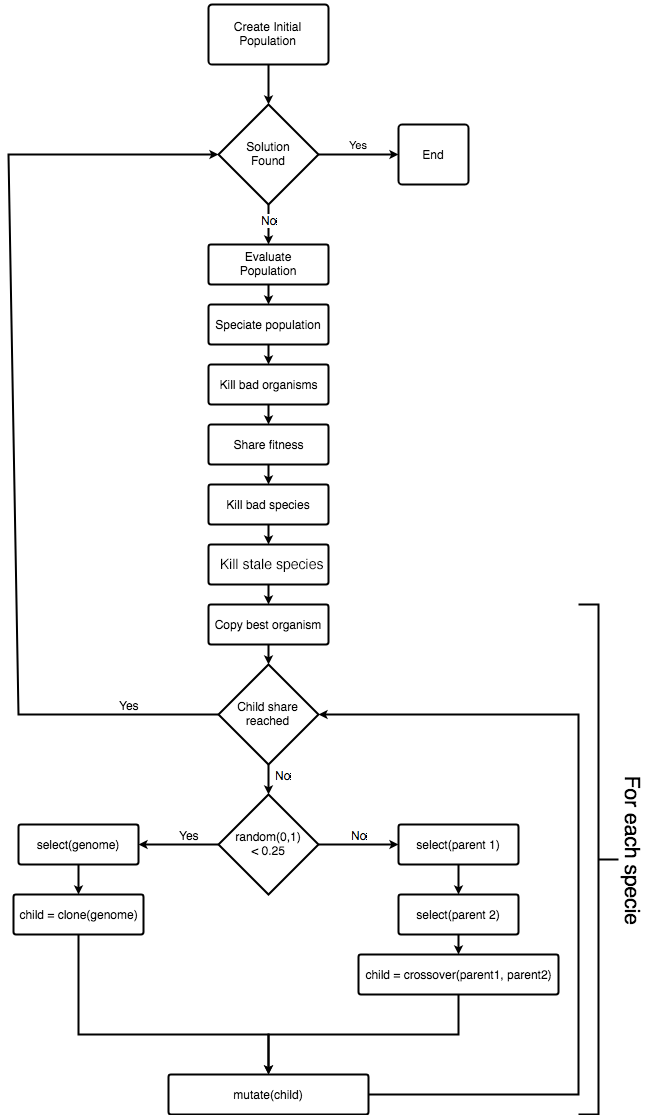
\includegraphics[scale=0.6]{neatflow.png}
\caption{Organigramme de l'algorithme NEAT}
\end{figure}
\clearpage
}
\newpage

\section{Architecture Réseau}

Afin d'optimiser la vitesse de calcul, un système distribué à été mis en place. Celui-ci repose sur une architecture client-serveur classique où le client effectue les simulations et le serveur gère les génomes et s'occupe de distribuer de manière équitable le travail entre tous les clients.\\

\begin{figure}[H]
\begin{center}
	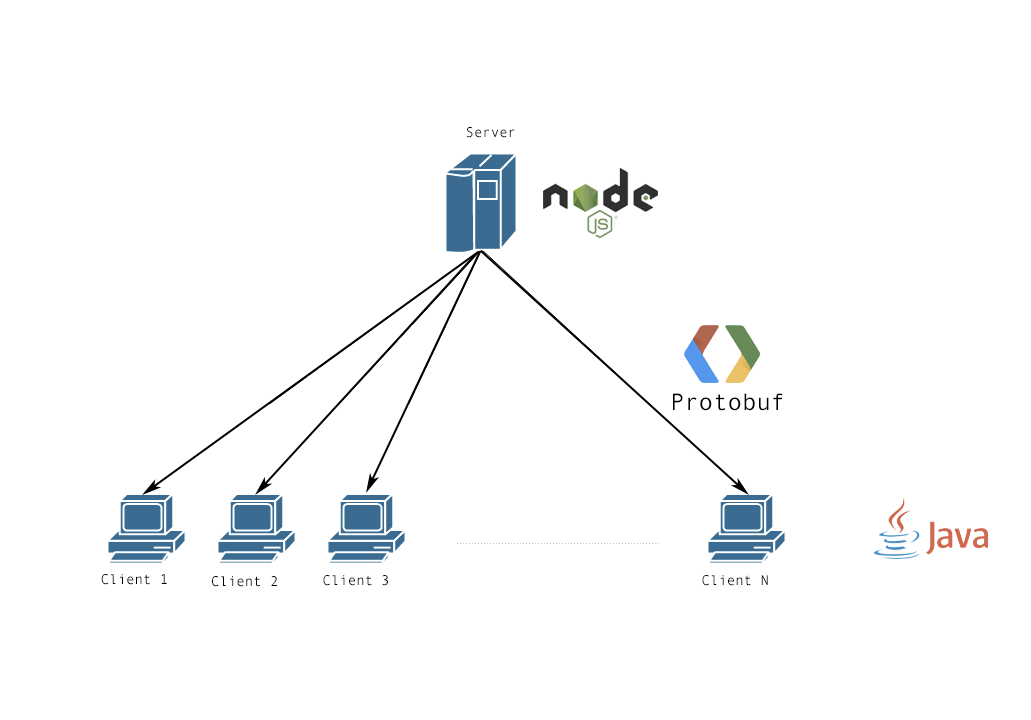
\includegraphics[scale=0.4]{archnet.png}
	\caption{Architecture réseau}
\end{center}
\end{figure}

\subsection{Protocole}

Le protocole à été établi à l'aide du langage protobuf qui permet d'avoir une définition claire ne dépendant pas des langages dans lesquels le protocole est ensuite implémenté.

Voici le fichier qui défini le protocole:
\inputminted[breaklines,breaksymbol=, frame=single,label=Protocole, stepnumber=1,tabsize=2]{protobuf}{mg.proto}

Le protocole définit donc 6 types de messages:
\begin{itemize}
\item MG\_JOIN, Envoyé par le client, c'est une demande à rejoindre le groupe de calcul. En paramètres sont donnés le nom du client et si il veut rejoindre en tant que specateur ou non (fonctionnalité expliquée dans la partie client).

\item MG\_JOIN\_RESPONSE, Envoyé par le serveur, confirme ou infirme l'ajout au groupe du client. Il n'existe pour l'instant aucune raison pour le rejet d'un client.

\item MG\_COMPUTE\_REQUEST, Envoyé par le serveur, demande au client de calculer le fitness d'un génome donné sur un jeu donné.

\item MG\_COMPUTE\_RESPONSE, Envoyé par le client, indique au serveur si oui ou non le client est en mesure d'effectuer la simulation.

\item MG\_COMPUTE\_RESULT, Envoyé par le client, donne le fitness obtenu par le génome donné dans le message MG\_COMPUTE\_REQUEST sur le jeu donné dans ce même message et le temps (ms) pris par le client pour effectuer la simulation.

\item MG\_END, Envoyé par n'importe quel entité, indique un désir de terminer la connexion.

\end{itemize}

\subsection{Serveur}

Comme écrit ci-dessus, le serveur à la lourde tâche de gérer tous les génomes et leurs fitness afin de mettre en oeuvre les algorithmes évolutionniste qui vont permettre l'évolution. En plus de cela il va également devoir servir les pages web servant à la gestion et à la surveillance du processus évolutif.\\
Afin de pouvoir effectuer toutes ces tâches, le serveur est constitué de modules node.js qui vont chacun gérer une partie de ce qui est lui est demandé.\\
L'architecture se présente ainsi:
\begin{figure}[H]
\begin{center}
	\includegraphics[scale=0.5]{"server.png"} 
	\caption{Architecture des modules du serveur}
\end{center}
\end{figure}

\subsection{Client}

Le client va devoir effectuer la simulation demandée par le serveur, avec le bon réseau de neurones

\subsubsection{Réseaux de neurones}
\subsubsection{Simulateur}
\subsubsection{Tests}

\newpage
\section{Interface de Controle}
\subsection{Mode}
\subsection{Tâche}
\subsection{Ouvriers}
\subsection{Graphs}

\newpage
\section{Base de donnés}

\newpage
\section{API}

\newpage
\section{Jeux}
\subsection{Asteroid}
\subsubsection{Principe}
\subsubsection{Entrées}
\subsubsection{Sorties}
\subsubsection{Résultats}

\newpage
\section{Conclusion}

\newpage
\bibliographystyle{unsrt}
\bibliography{mg}
\end{document}
